% This is "sig-alternate.tex" V2.1 April 2013
% This file should be compiled with V2.5 of "sig-alternate.cls" May 2012
%
% This example file demonstrates the use of the 'sig-alternate.cls'
% V2.5 LaTeX2e document class file. It is for those submitting
% articles to ACM Conference Proceedings WHO DO NOT WISH TO
% STRICTLY ADHERE TO THE SIGS (PUBS-BOARD-ENDORSED) STYLE.
% The 'sig-alternate.cls' file will produce a similar-looking,
% albeit, 'tighter' paper resulting in, invariably, fewer pages.
%
% ----------------------------------------------------------------------------------------------------------------
% This .tex file (and associated .cls V2.5) produces:
%       1) The Permission Statement
%       2) The Conference (location) Info information
%       3) The Copyright Line with ACM data
%       4) NO page numbers
%
% as against the acm_proc_article-sp.cls file which
% DOES NOT produce 1) thru' 3) above.
%
% Using 'sig-alternate.cls' you have control, however, from within
% the source .tex file, over both the CopyrightYear
% (defaulted to 200X) and the ACM Copyright Data
% (defaulted to X-XXXXX-XX-X/XX/XX).
% e.g.
% \CopyrightYear{2007} will cause 2007 to appear in the copyright line.
% \crdata{0-12345-67-8/90/12} will cause 0-12345-67-8/90/12 to appear in the copyright line.
%
% ---------------------------------------------------------------------------------------------------------------
% This .tex source is an example which *does* use
% the .bib file (from which the .bbl file % is produced).
% REMEMBER HOWEVER: After having produced the .bbl file,
% and prior to final submission, you *NEED* to 'insert'
% your .bbl file into your source .tex file so as to provide
% ONE 'self-contained' source file.
%
% ================= IF YOU HAVE QUESTIONS =======================
% Questions regarding the SIGS styles, SIGS policies and
% procedures, Conferences etc. should be sent to
% Adrienne Griscti (griscti@acm.org)
%
% Technical questions _only_ to
% Gerald Murray (murray@hq.acm.org)
% ===============================================================
%
% For tracking purposes - this is V2.0 - May 2012

\documentclass{sig-alternate-05-2015}

\usepackage{epstopdf}
\usepackage{float}
\usepackage{graphicx}
\usepackage{amsmath}


\begin{document}

% Copyright
%\setcopyright{acmcopyright}
%\setcopyright{acmlicensed}
%\setcopyright{rightsretained}
%\setcopyright{usgov}
%\setcopyright{usgovmixed}
%\setcopyright{cagov}
%\setcopyright{cagovmixed}


% DOI
%\doi{10.475/123_4}

% ISBN
%\isbn{123-4567-24-567/08/06}

%Conference
%\conferenceinfo{PLDI '13}{June 16--19, 2013, Seattle, WA, USA}

%\acmPrice{\$15.00}

%
% --- Author Metadata here ---
%\conferenceinfo{WOODSTOCK}{'97 El Paso, Texas USA}
%\CopyrightYear{2007} % Allows default copyright year (20XX) to be over-ridden - IF NEED BE.
%\crdata{0-12345-67-8/90/01}  % Allows default copyright data (0-89791-88-6/97/05) to be over-ridden - IF NEED BE.
% --- End of Author Metadata ---

\title{CSE 847 Project Proposal}
\subtitle{Yinyang K-means}
%\titlenote{A full version of this paper is available as
%\textit{Author's Guide to Preparing ACM SIG Proceedings Using
%\LaTeX$2_\epsilon$\ and BibTeX} at
%\texttt{www.acm.org/eaddress.htm}}}
%
% You need the command \numberofauthors to handle the 'placement
% and alignment' of the authors beneath the title.
%
% For aesthetic reasons, we recommend 'three authors at a time'
% i.e. three 'name/affiliation blocks' be placed beneath the title.
%
% NOTE: You are NOT restricted in how many 'rows' of
% "name/affiliations" may appear. We just ask that you restrict
% the number of 'columns' to three.
%
% Because of the available 'opening page real-estate'
% we ask you to refrain from putting more than six authors
% (two rows with three columns) beneath the article title.
% More than six makes the first-page appear very cluttered indeed.
%
% Use the \alignauthor commands to handle the names
% and affiliations for an 'aesthetic maximum' of six authors.
% Add names, affiliations, addresses for
% the seventh etc. author(s) as the argument for the
% \additionalauthors command.
% These 'additional authors' will be output/set for you
% without further effort on your part as the last section in
% the body of your article BEFORE References or any Appendices.

\numberofauthors{2} %  in this sample file, there are a *total*
% of EIGHT authors. SIX appear on the 'first-page' (for formatting
% reasons) and the remaining two appear in the \additionalauthors section.
%
\author{
% You can go ahead and credit any number of authors here,
% e.g. one 'row of three' or two rows (consisting of one row of three
% and a second row of one, two or three).
%
% The command \alignauthor (no curly braces needed) should
% precede each author name, affiliation/snail-mail address and
% e-mail address. Additionally, tag each line of
% affiliation/address with \affaddr, and tag the
% e-mail address with \email.
%
% 1st. author
\alignauthor
Ben Frey\\
       \email{freybenj@msu.edu}
% 2nd. author
\alignauthor
Thomas Swearingen\\
       \email{swearin3@msu.edu}
}
% There's nothing stopping you putting the seventh, eighth, etc.
% author on the opening page (as the 'third row') but we ask,
% for aesthetic reasons that you place these 'additional authors'
% in the \additional authors block, viz.
%\additionalauthors{Additional authors: John Smith (The Th{\o}rv{\"a}ld Group,
%email: {\texttt{jsmith@affiliation.org}}) and Julius P.~Kumquat
%(The Kumquat Consortium, email: {\texttt{jpkumquat@consortium.net}}).}
%\date{30 July 1999}
% Just remember to make sure that the TOTAL number of authors
% is the number that will appear on the first page PLUS the
% number that will appear in the \additionalauthors section.

\maketitle
%\begin{abstract}
%Abstract goes here.
%\end{abstract}


%
% The code below should be generated by the tool at
% http://dl.acm.org/ccs.cfm
% Please copy and paste the code instead of the example below. 
%
%\begin{CCSXML}
%<ccs2012>
% <concept>
%  <concept_id>10010520.10010553.10010562</concept_id>
%  <concept_desc>Computer systems organization~Embedded systems</concept_desc>
%  <concept_significance>500</concept_significance>
% </concept>
% <concept>
%  <concept_id>10010520.10010575.10010755</concept_id>
%  <concept_desc>Computer systems organization~Redundancy</concept_desc>
%  <concept_significance>300</concept_significance>
% </concept>
% <concept>
%  <concept_id>10010520.10010553.10010554</concept_id>
%  <concept_desc>Computer systems organization~Robotics</concept_desc>
%  <concept_significance>100</concept_significance>
% </concept>
% <concept>
%  <concept_id>10003033.10003083.10003095</concept_id>
%  <concept_desc>Networks~Network reliability</concept_desc>
%  <concept_significance>100</concept_significance>
% </concept>
%</ccs2012>  
%\end{CCSXML}

%\ccsdesc[500]{Computer systems organization~Embedded systems}
%\ccsdesc[300]{Computer systems organization~Redundancy}
%\ccsdesc{Computer systems organization~Robotics}
%\ccsdesc[100]{Networks~Network reliability}


%
% End generated code
%

%
%  Use this command to print the description
%
%\printccsdesc

% We no longer use \terms command
%\terms{Theory}

%\keywords{ACM proceedings; \LaTeX; text tagging}

\section{Problem Description}

K-means is a popular machine learning algorithm for clustering.
As the amount of data has grown ever larger, the limitation of the classic K-mean algorithm has become more apparent.
Specifically, the K-means algorithm is linear in data set size---the number of distance calculations is nki, where n is the number of data points, k is the number of desired clusters, and i is the number of iterations.
This linearity reduces the usability of the algorithm with large datasets.
However, Ding \textit{et al.} propose Yinyang K-means \cite{Ding2015} which seeks to solve this problem.
The authors assert Yinyang K-means can be used in place of classical K-means with no extra conditions or requirements while simultaneously achieving an order of magnitude higher performance.
We intend to explore the theoretical properties of this proposed method and verify the authors' claim of a significant speed up.

\section{Introduction}

K-means is a venerable clustering algorithm which has gained the trust of researchers through years of use.
However, when the dimensionality, data set size, or number of desired clusters is large, k-means becomes prohibitively expensive.
Attempts at increasing the performance of k-means mainly fall into two categories: working on improving the core algorithm or improving the performance through some other means (e.g. K-means++ \cite{Arthur2007}).
This work focuses on the former method, which includes approximation and optimization.
Within this realm, work has been done previously on structural or incremental optimization by \cite{Pelleg1999}, \cite{Elkan2003}, and \cite{Drake2012} and on approximation by several groups (\cite{Guha1998}, \cite{Czumaj2007}), \cite{Philbin2007}, \cite{Sculley2010}, \cite{Wang2015}).
While this previous work has been of high quality, none of the innovations have gotten much traction or widespread use.

In \textit{Drake and Hamerly} \cite{Drake2012}, the authors keep $b$ lower bounds, where $b<k$, $k$ being the number of bounds kept in \textit{Elkan} \cite{Elkan2003}.
These bounds are the distances to the $b$ nearest neighbors of the point in question, and are kept by tracking a point's center and the $1\leq z\leq b$ closest centers.
Of particular note, \textit{Drake and Hamerly} tune $b$ adaptively as follows: start at $b=\frac{k}{4}$; after each iteration, $b$ becomes the number of useful bounds while staying at least $\frac{k}{8}$.

It has been hypothesized that in order to gain popularity in practical use, a replacement for k-means must meet three requirements: equivalent clustering to traditional k-means, consistent and significant performance gains, and simple to use.

The proposed work aims to satisfy those three requirements.
It utilizes the triangle inequality in a novel way to keep track of two bounds: the upper bound on the distance from a given point to its assigned cluster center and the lower bound on the distance from the point to any other center.
These two bounds act to reduce the number of distance calculations that need to be performed during the assignment step of k-means.
This is achieved through two kinds of filtering: group/global filtering and local filtering.
Global filtering works to determine if a point needs to be assigned to a different cluster based on the movement of the cluster centers.
If centers change by a large amount, then it is more likely that points need their cluster assignment checked.
Group filtering generalizes the global filtering by initially grouping the clusters into groups before the first iteration of k-means and applying the global filter to those groups.
Local filtering is performed on any groups of cluster centers that make it through the group filter.
Centers that get filtered by the local filter do not have their distances to the data points calculated.

Additionally, a method to optimize the second step of k-means, the center update step, is proposed.
The new method updates the cluster centers by modifying them, rather than calculating the average across all points contained in that cluster.

\section{Preliminary Plan}

The theory thrust of the project consist of 3 requirements and a 4th optional task:

\begin{itemize}
\item Show all details of the proof of correctness
\item Implement the algorithm
\item Test algorithm on synthetic dataset to verify theoretical properties
\item \textit{Test algorithm on a real-world dataset}
\end{itemize}

Figure \ref{fig:timeline} shows the overview of our project timeline.
We first plan to write up the introduction and problem description that will be included in the intermediate project report and the final project report.
This document includes the first draft of those sections.
We will expand on them over time to give a thorough description of the work and place it in the context of other related works.

\begin{figure*}[t]
    \centering
    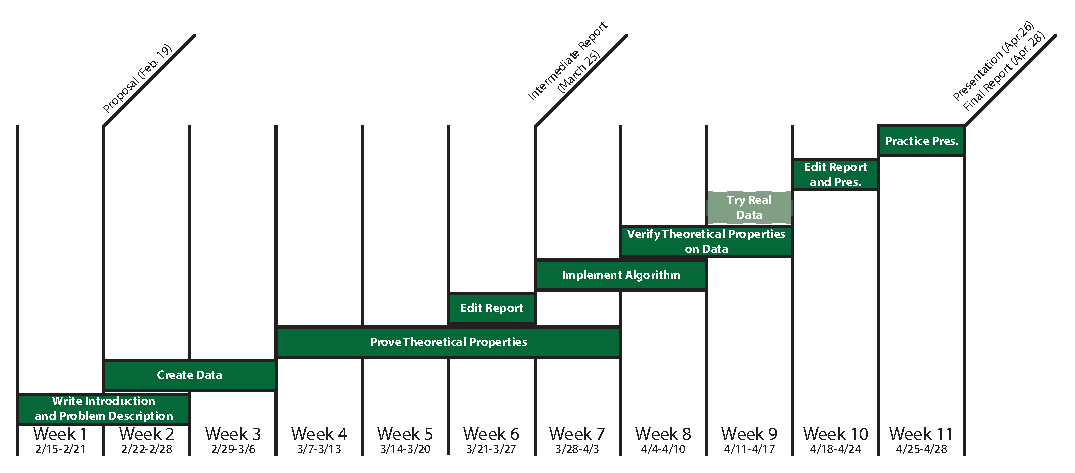
\includegraphics[width=\textwidth]{figures/timeline.eps}
    \caption{Project timeline showing key steps in the project. A solid color border indicates required step while a dotted line border indicates an optional step that will only be completed if there is time.}
    \label{fig:timeline}
\end{figure*}

Once we have a thorough understanding of the problem and the algorithm, we can generate data which will test the algorithm.
The synthetic data should push the limits of the algorithm.
Since the authors intend for Yinyang K-means to extend classic K-means to better cope with large datasets, then the synthetic data should be quite large as well.

The next step is proving the theoretical properties of Yinyang K-means.
This includes the Global-Filtering Condition and the Local-Filtering Condition.
The Global-Filtering Condition asserts that cluster assignment of a point is only necessary if the cluster centroid changes drastically.
The Local-Filtering Condition allows skipping distance calculations between a point and a centroid if that point is with some set distance to another centroid.
We will also investigate the authors' claim that Yinyang K-means achieves the same performance as classic K-means with an order of magnitude performance increase.

The last part of the project involves implementing the algorithm on a computer.
Once it is implemented and verified to be correct, we can then test the algorithm on the synthetic data we generated earlier.
The synthetic data will be created in a such a way that the theoretical properties of the algorithm will be tested.
This will tell us that these properties actually hold in practice.
If there is time, we also plan to try the algorithm on a real-world dataset which will hopefully see the same benefits as the synthetic data.



%
% The following two commands are all you need in the
% initial runs of your .tex file to
% produce the bibliography for the citations in your paper.
\bibliographystyle{abbrv}
\bibliography{yinyang}  % sigproc.bib is the name of the Bibliography in this case
% You must have a proper ".bib" file
%  and remember to run:
% latex bibtex latex latex
% to resolve all references
%
% ACM needs 'a single self-contained file'!
%
%APPENDICES are optional
%\balancecolumns
%\appendix
%Appendix A
%\section{Headings in Appendices}

\end{document}
